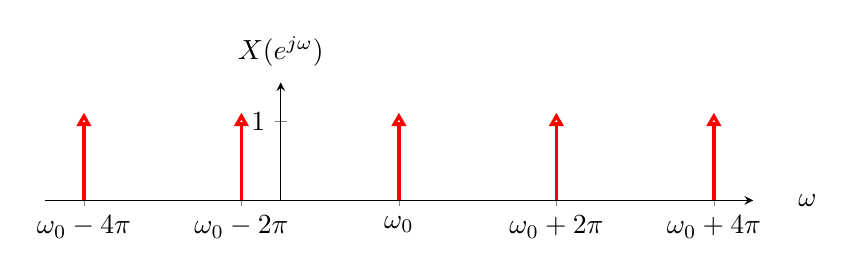
\begin{tikzpicture}[scale=1]	


    \begin{axis}[
    		name=axis1,
		y=1cm,
		x=0.5cm,
		 clip=false,
		 xmin=-6,xmax=12,
		 xlabel= $\omega$,
		 ylabel={$X(e^{j\omega})$},
		 ymin=0,ymax=1.5,
		 axis lines=middle,
         	xtick={-5, -1, 3, 7, 11},
         	xticklabels={$\omega_0 -4\pi$, $\omega_0 -2\pi$, $\omega_0$, $\omega_0 + 2\pi$, $\omega_0 +4\pi$},
		 ytick={1},
		 yticklabels={1},
		 every axis x label/.style={at={(ticklabel* cs:1.05)}, anchor=west,},
		every axis y label/.style={at={(ticklabel* cs:1.05)}, anchor=south,},
     ]
	\addplot[ycomb, mark=triangle,mark options={rotate=0}, very thick, red] plot coordinates {(-5,1) (-1,1) (3,1) (7,1) (11,1)};

    \end{axis}


%     \begin{axis}[
%     	name=axis2,
%     	at={($(axis1.south east)+(0,-1.1cm)$)},anchor=north east,
% 		y=1cm,
% 		x=1cm,
% 		 clip=false,
% 		 xmin=-3.5,xmax=10,
% 		 xlabel= $\omega$,
% 		 ylabel={$Na_k$},
% 		 ymin=-1.5,ymax=6,
% 		 axis lines=middle,
%          	xtick={-3.1416, 3.1416, 6.2832},
%          	xticklabels={$-\pi$, $\pi$, $2\pi$},
% 		 %ytick={-1, 1},
% 		 yticklabels=\empty,
% 		 every axis x label/.style={at={(ticklabel* cs:1.05)}, anchor=west,},
% 		every axis y label/.style={at={(ticklabel* cs:1.05)}, anchor=south,},
%      ]
% 		\addplot [red, smooth, mark=none] table [x={o}, y={xo}] {./g_dt_fs/figures/dtfs_square_N20.dat};
% 		\addplot [blue, ycomb, mark=*] table [x={o}, y={xo}] {./g_dt_fs/figures/dtfs_square_stem_N20.dat};
% 
% 		\node at (axis cs:10, 3) [anchor=east] { $N=20$ };
%     \end{axis}



\end{tikzpicture} 